\chapter{Durchführung}

\section{Versuchsaufbau}
Für den Versuch wurden folgende Geräte und Materialien verwendet:
\begin{itemize}
  \item Wasserkalorimeter mit Magnetrührer
  \item Elektrischer Kocher mit Glasbecher
  \item Dewargefäß für flüssigen Stickstoff
  \item Elektronisches Thermometer
  \item Elektronische Waage
  \item Stoppuhr
  \item Stativ mit Drahthaken
  \item Schutzbrille und Schutzhandschuhe
  \item Große/Kleine Testkörper aus Graphit, Aluminium, Blei
\end{itemize}


\begin{figure}[h!]
    \centering
    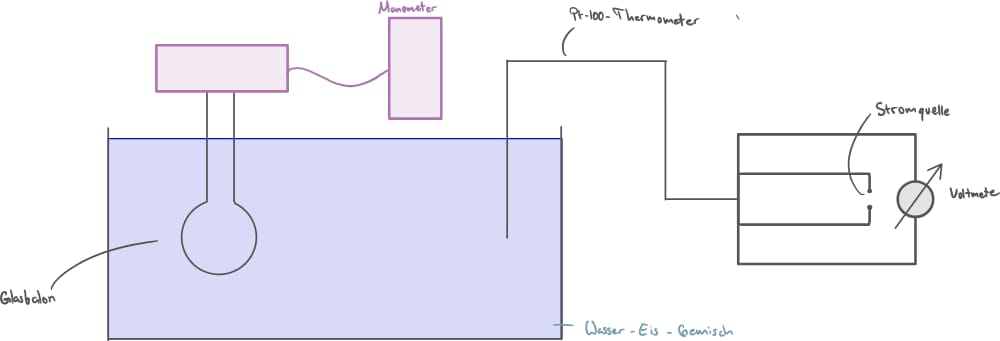
\includegraphics[width=0.35\textwidth]{img/\versuchsnummer/1.jpg}
    \caption{Wasserbecher auf Heizplatte mit Rüherfisch und Thermometer zur Temperaturkontrolle}
    \label{img:1}
\end{figure}

\newpage


\section{Messverfahren}
\subsection*{Wasserkalorimeter}
Die Bestimmung der Wärmekapazität im Bereich von \SI{20}{\celsius} bis \SI{100}{\celsius} erfolgt mit der Mischungsmethode.  
Ein Probekörper wird in kochendem Wasser auf Temperatur \(T_1\) gebracht und anschließend in das Kalorimeter mit Wasser der Temperatur \(T_2\) überführt. Nach Einstellung der Gleichgewichtstemperatur \(T\) lässt sich \(c_x\) mit \hyperref[eq:spezifische_kalorimeter]{Gleichung \ref*{eq:spezifische_kalorimeter}} berechnen.  

Zur Bestimmung des Wasserwerts \(W\) wird ein separates Experiment durchgeführt, siehe \hyperref[eq:wasserwert]{Gleichung \ref*{eq:wasserwert}}.
\begin{figure}[h!]
    \centering
    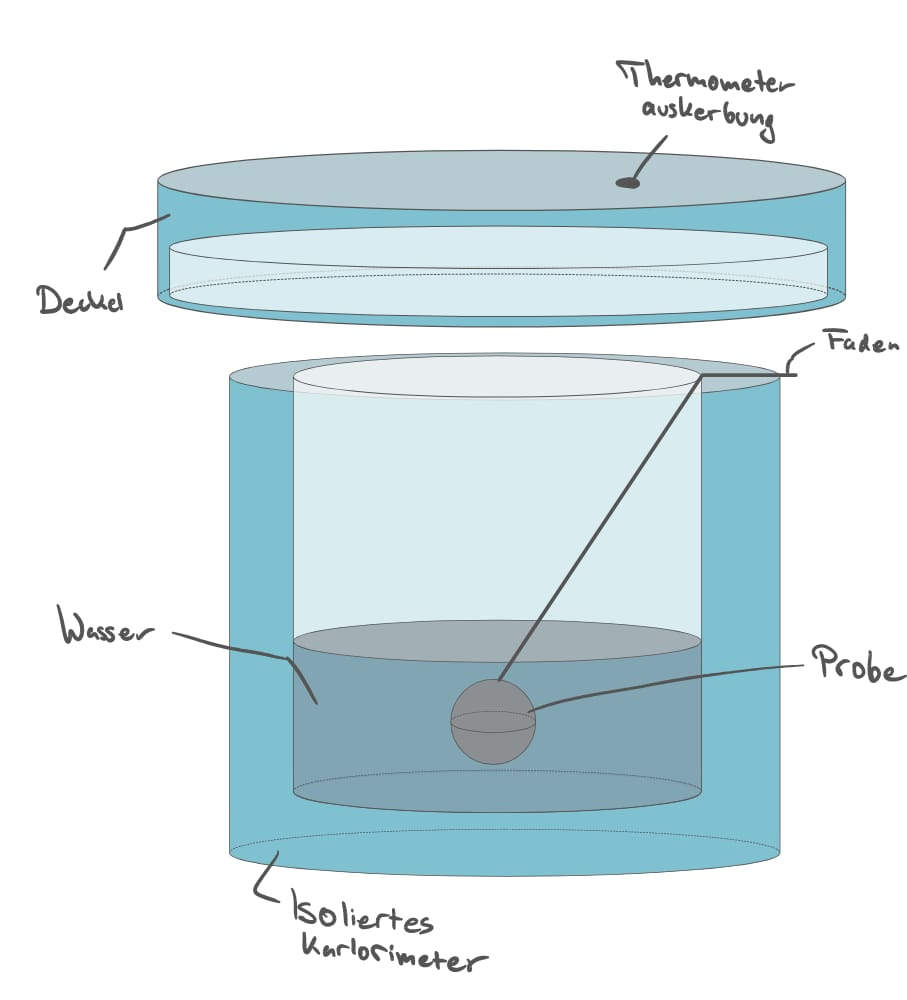
\includegraphics[width=0.35\textwidth]{img/\versuchsnummer/2.jpg}
    \caption{Schematische Darstellung des Wasserkalorimeters}
    \label{img:2}
\end{figure}

\subsection*{Flüssiger Stickstoff}
Für tiefe Temperaturen wird ein kleiner Testkörper mit Temperatur \(T_1\) in ein Dewargefäß mit flüssigem Stickstoff (\(T_2 \approx \SI{-195.8}{\celsius}\)) eingebracht. Die Masse des verdampften Stickstoffs \(m_V\) wird durch Wiegen des Dewargefäßes vor und nach dem Versuch bestimmt.  

Mit der Verdampfungswärme \(Q_V\) folgt aus \hyperref[eq:stickstoff_cx]{Gleichung \ref*{eq:stickstoff_cx}} die spezifische Wärmekapazität des Festkörpers.  

Die Messung wird für Graphit, Aluminium und Blei durchgeführt. Parallel werden Raumtemperatur und Atmosphärendruck protokolliert.
\begin{figure}[h!]
    \centering
    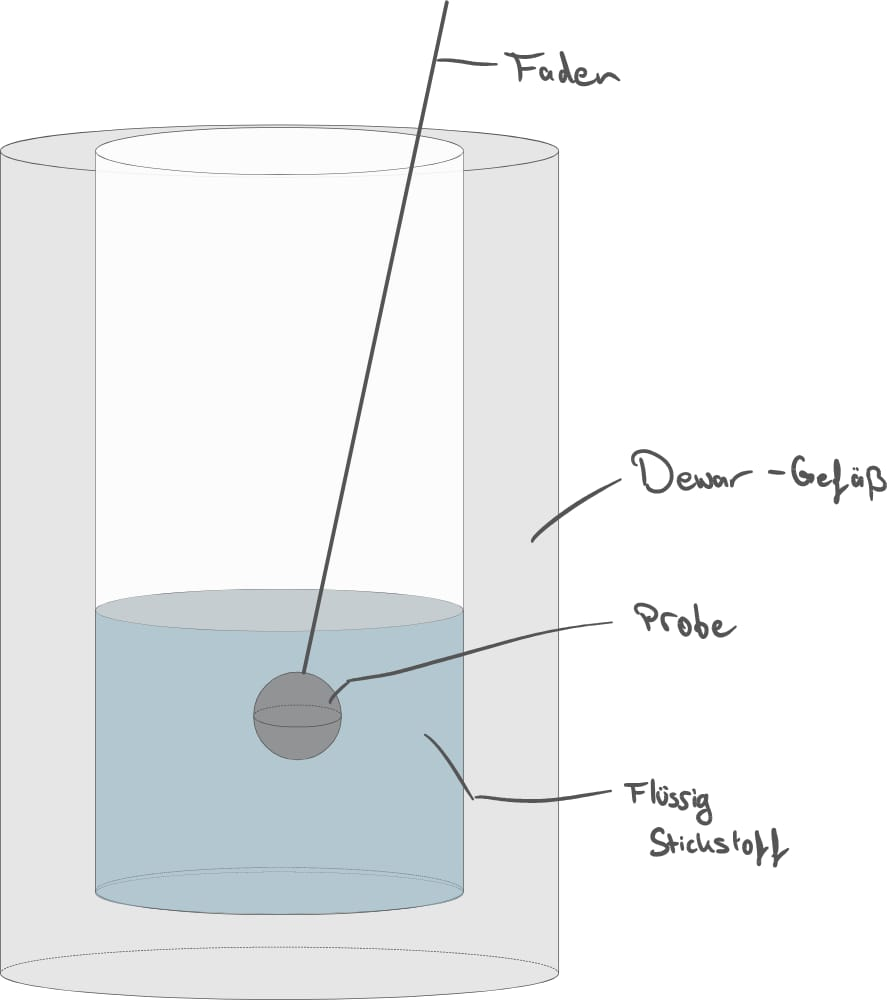
\includegraphics[width=0.35\textwidth]{img/\versuchsnummer/3.jpg}
    \caption{Dewargefäß}
    \label{img:3}
\end{figure}